% ****** Start of file apssamp.tex ******
%
%   This file is part of the APS files in the REVTeX 4.2 distribution.
%   Version 4.2a of REVTeX, December 2014
%
%   Copyright (c) 2014 The American Physical Society.
%
%   See the REVTeX 4 README file for restrictions and more information.
%
% TeX'ing this file requires that you have AMS-LaTeX 2.0 installed
% as well as the rest of the prerequisites for REVTeX 4.2
%
% See the REVTeX 4 README file
% It also requires running BibTeX. The commands are as follows:
%
%  1)  latex apssamp.tex
%  2)  bibtex apssamp
%  3)  latex apssamp.tex
%  4)  latex apssamp.tex
%
\documentclass[%
 reprint,
%superscriptaddress,
%groupedaddress,
%unsortedaddress,
%runinaddress,
%frontmatterverbose, 
%preprint,
%preprintnumbers,
%nofootinbib,
%nobibnotes,
%bibnotes,
 amsmath,amssymb,
 aps,
%pra,
%prb,
%rmp,
%prstab,
%prstper,
%floatfix,
]{revtex4-2}

\usepackage{graphicx}% Include figure files
\usepackage{dcolumn}% Align table columns on decimal point
\usepackage{bm}% bold math
\usepackage[font=scriptsize,labelfont=bf, justification=justified]{caption}% change fontsize in captions
\usepackage{booktabs}
\usepackage{subfigure}
%\usepackage{hyperref}% add hypertext capabilities
%\usepackage[mathlines]{lineno}% Enable numbering of text and display math
%\linenumbers\relax % Commence numbering lines

%\usepackage[showframe,%Uncomment any one of the following lines to test 
%%scale=0.7, marginratio={1:1, 2:3}, ignoreall,% default settings
%%text={7in,10in},centering,
%%margin=1.5in,
%%total={6.5in,8.75in}, top=1.2in, left=0.9in, includefoot,
%%height=10in,a5paper,hmargin={3cm,0.8in},
%]{geometry}

\begin{document}

\preprint{APS/123-QED}

\title{PHYC40600 - Physics with Astronomy and Space Science Lab 2;\\\vspace{1cm}555 Timer and Raspberry Pi Pico Pulse-Width Modulation}

\author{Daragh Hollman}
\affiliation{%
 daragh.hollman@ucdconnect.ie
}%

\date{\today}% It is always \today, today,
             %  but any date may be explicitly specified

\begin{abstract}
\end{abstract}

\maketitle

\section{Introduction}

    Pulse width modulation (PWM) is a useful technique for controlling analog circuits digitally. Through the use of high-resolution internal counters, the duty cycle (the ratio of time the signal is on compared to off) of a square wave can be modulated to reduce the average power supplied to a load to a specific analog signal level \cite{barr}. The result is an analogue signal with amplitude at any given time proportional to the width of the pulse. An example PWM signal is shown in figure \ref{fig:PWM} for varying duty cycle. This switching is usually done at high frequencies so no discernible flickering is observed in the power delivery \cite{ucd}.\\

    Applications of PWM begin with simply adjusting the brightness of lights but extend to less obvious use cases such as in the motor power regulation of light rail (such as the LUAS in Dublin \cite{ucd}) and in AM radio transmission \cite{radioworld}.\\

    \begin{figure}
        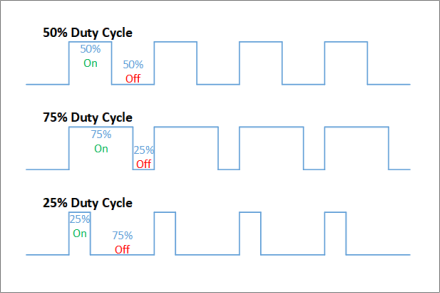
\includegraphics[width=0.9\columnwidth]{Images/pwm.png}
        \caption{\label{fig:PWM}Examples of difference duty cycles for a square wave \cite{ucd}.}
    \end{figure}

    The 555 Timer is a...


\section{PWM with a Raspberry Pi Pico}
The Raspberry Pi Pico is a high-performance microcontroller with multi-function digital I/O pins \cite{Pi, ucd}. PWM is one of these functions. A pin diagram along with full documentation can be found at \url{https://www.raspberrypi.com/documentation/microcontrollers/raspberry-pi-pico.html} \cite{Pi}. For ease of reading, this pin diagram is also included in appendix 1.\\

The Pi Pico can be programmed using an implementation of Python 3 designed to run optimally on microcontrollers and other small or otherwise constrained environments called MicroPython \cite{micropython}. MicroPython contains the \textsc{machine} library from which the \textsc{PWM} function can be used to generate a PWM output on a designated pin. The frequency of the PWM can be set up to frequencies beyond $1\,\text{MHz}$, however in this lab we only use up to a maximum $100 \,\text{kHz}$ \cite{ucd}. The duty cycle can be set to an integer value between $0$ and $65535$ (the 16-bit binary maximum), with the ratio of this value and the maximum yielding the ratio the signal will be on compared to off.\\

In this section, we first verify the PWM generation from the Pi Pico behaves as expected, and then design scripts to adjust the brightness of the inbuilt LED on the microcontroller. Following this, the combination of the PWM output and a low pass filter will be used to create a simple Digital-To-Analogue Converter (DAC). Lastly, the generation of analogue signals will be described and demonstrated for a triangle and sine wave.
    
    \subsection{Basics}
    To first verify the PWM output from the Pi Pico, a simple script was written to output PWM for a constant frequency and duty. The output of this pin was measured with an oscilloscope and recorded for several duty values with a constant frequency, and also for several frequency values for a constant duty value. Variations in duty are plotted in figure \ref{fig:constFreq}, and variations in frequency are plotted in figure \ref{fig:constDuty}. We can see that the PWM output is what is expected by comparison with figure \ref{fig:PWM}. Frequency adjusts the frequency of the square wave output as a whole, while duty adjusts the amount the square wave is on compared to off.\\

    \begin{figure}
        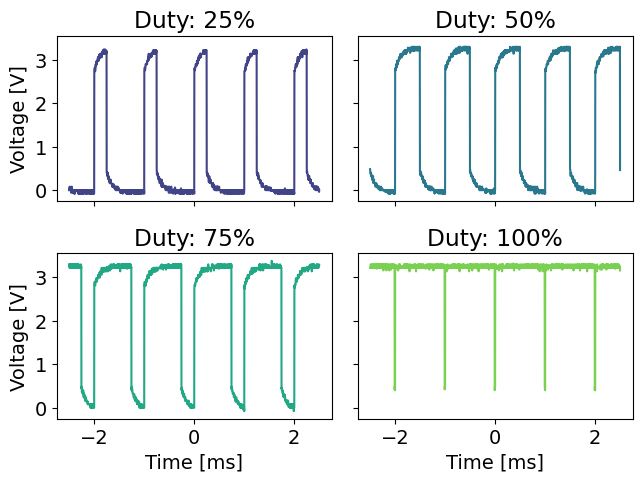
\includegraphics[width=0.9\columnwidth]{Images/constFreq.png}
        \caption{\label{fig:constFreq}PWM output from the Pi Pico showing variations in duty for a constant frequency of $1000 \,\text{Hz}$}
    \end{figure}
    \begin{figure}
        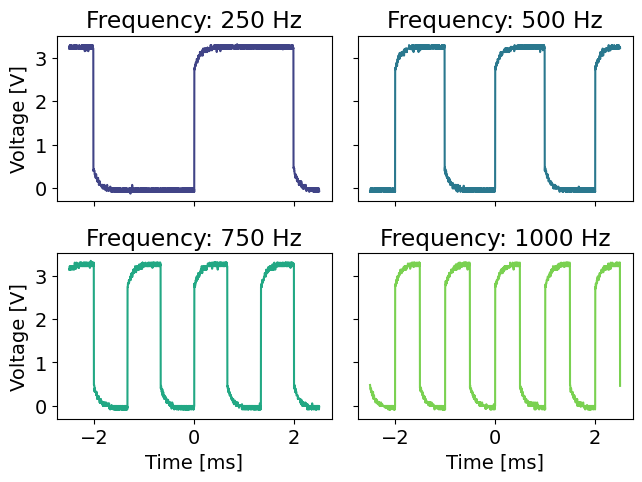
\includegraphics[width=0.9\columnwidth]{Images/constDuty.png}
        \caption{\label{fig:constDuty}PWM output from the Pi Pico showing variations in frequency for a constant duty of $\approx 50$\% (i.e. $65535/2 \approx 32768$, rounding to an integer value.)}
    \end{figure}

    Instead of passing the PWM output to an oscilloscope, the output was sent to internal LED on the Pi Pico (GPIO pin 25, see pin diagram). A \textit{brightness value} float between $0$ (off) and $1$ (full brightness) was defined in the script mentioned previously. The simple multiplication of this brightness value with the maximum duty value $65535$ is sufficient to control the brightness of the LED from this variable. Note that the duty value must be rounded to an integer as this floating point multiplication will result in decimal values which the Pi Pico cannot receive. For low PWM frequencies, flickering of the LED could be observed (as briefly mentioned in the introduction). A 2014 study report that the minimum viewing time required for visual comprehension could be as low as $13\,\text{ms}$ per frame in a sequence \cite{potter_2014}. This corresponds to a minimum frequency $75 \,\text{Hz}$. This value is decisively on the upper end of human capabilities (and is described as such in the study which quotes findings between $13\,\text{ms}$ and $80\,\text{ms}$), given a common monitor refresh rate of $60\,\text{Hz}$ or higher for modern devices \cite{refresh}. To avoid visible flickering in our LED, a higher frequency of $100 \,\text{Hz}$ was chosen.\\

    From here, it is easy to adjust this brightness value over time to linearly transition between $0$ and $1$. A loop was created to increase the brightness in steps of 0.01 for 100 steps, and then decrease again by the same value for a total length of 200 steps. In each step, a small delay $\mathcal{O}(\text{ms})$ could be applied to define the length of time to cycle through the loop. This delay $t_\text{delay}$ was defined as follows:
    \begin{equation}
        t_\text{delay} = \text{round}_\text{ms}\left( \frac{\text{period}}{\text{N}} \right)
    \end{equation}where the period is the length of time for one full cycle, and $N$ the number of steps in the cycle, all rounded to the nearest millisecond.\\

    Observing the LED it is clear that while the brightness value is being incremented linearly, the light does not appear to change linearly in brightness. It appears to stay brighter for longer than it is dimmer. This is however expected, as we know that the human eye has a logarithmic response to changes in light intensity. This phenomenon is part of what is known as the Weber-Fechner Laws \cite{maes_2021}. We can adjust for this, by increasing and decreasing the brightness linearly in log-space. This was not fully achieved for this exercise but a close approximation was implemented which was functionally similar. The brightness was increased with the following equation:
    \begin{equation}
        10^{t} \over 10
    \end{equation}and decreased with:
    \begin{equation}
        10^{-(t+1)} \over 10
    \end{equation}where $t$ is the position along the respective half of the 200 step cycle from $0$ to $1$, i.e. $i/100$ where $i$ is the step number. While effective in producing a increase linear in log space, these equations do have the drawback of their bounds. The minimum value, corresponding to $t=0$ for each is only at $10$\% of the maximum brightness, and as such the LED will never reach the fully off state. Despite the constraints on the range, the LED was observed to range between the two brightness values linearly (to the eye). The script for producing both of these effects is included in appendix 2.


    \subsection{Simple DAC}

    \subsection{Generating Analogue Output Functions}

        \subsubsection{Triangular Signal}

        \subsubsection{Sine Wave}


\section{555 Timer}
    
    \subsection{555 Timer as an Astable Oscillator}

        \subsubsection{Simulations}

        \subsubsection{Circuit Construction}


    \subsection{Designing a Time-To-Amplitude Converter utilising the 555 Timer}


\clearpage
\bibliographystyle{unsrt}
\bibliography{aps_references}% Produces the bibliography via BibTeX

\clearpage
\onecolumngrid
\appendix

\section{Pi Pico Pin Diagram}

    \begin{figure}[h]
        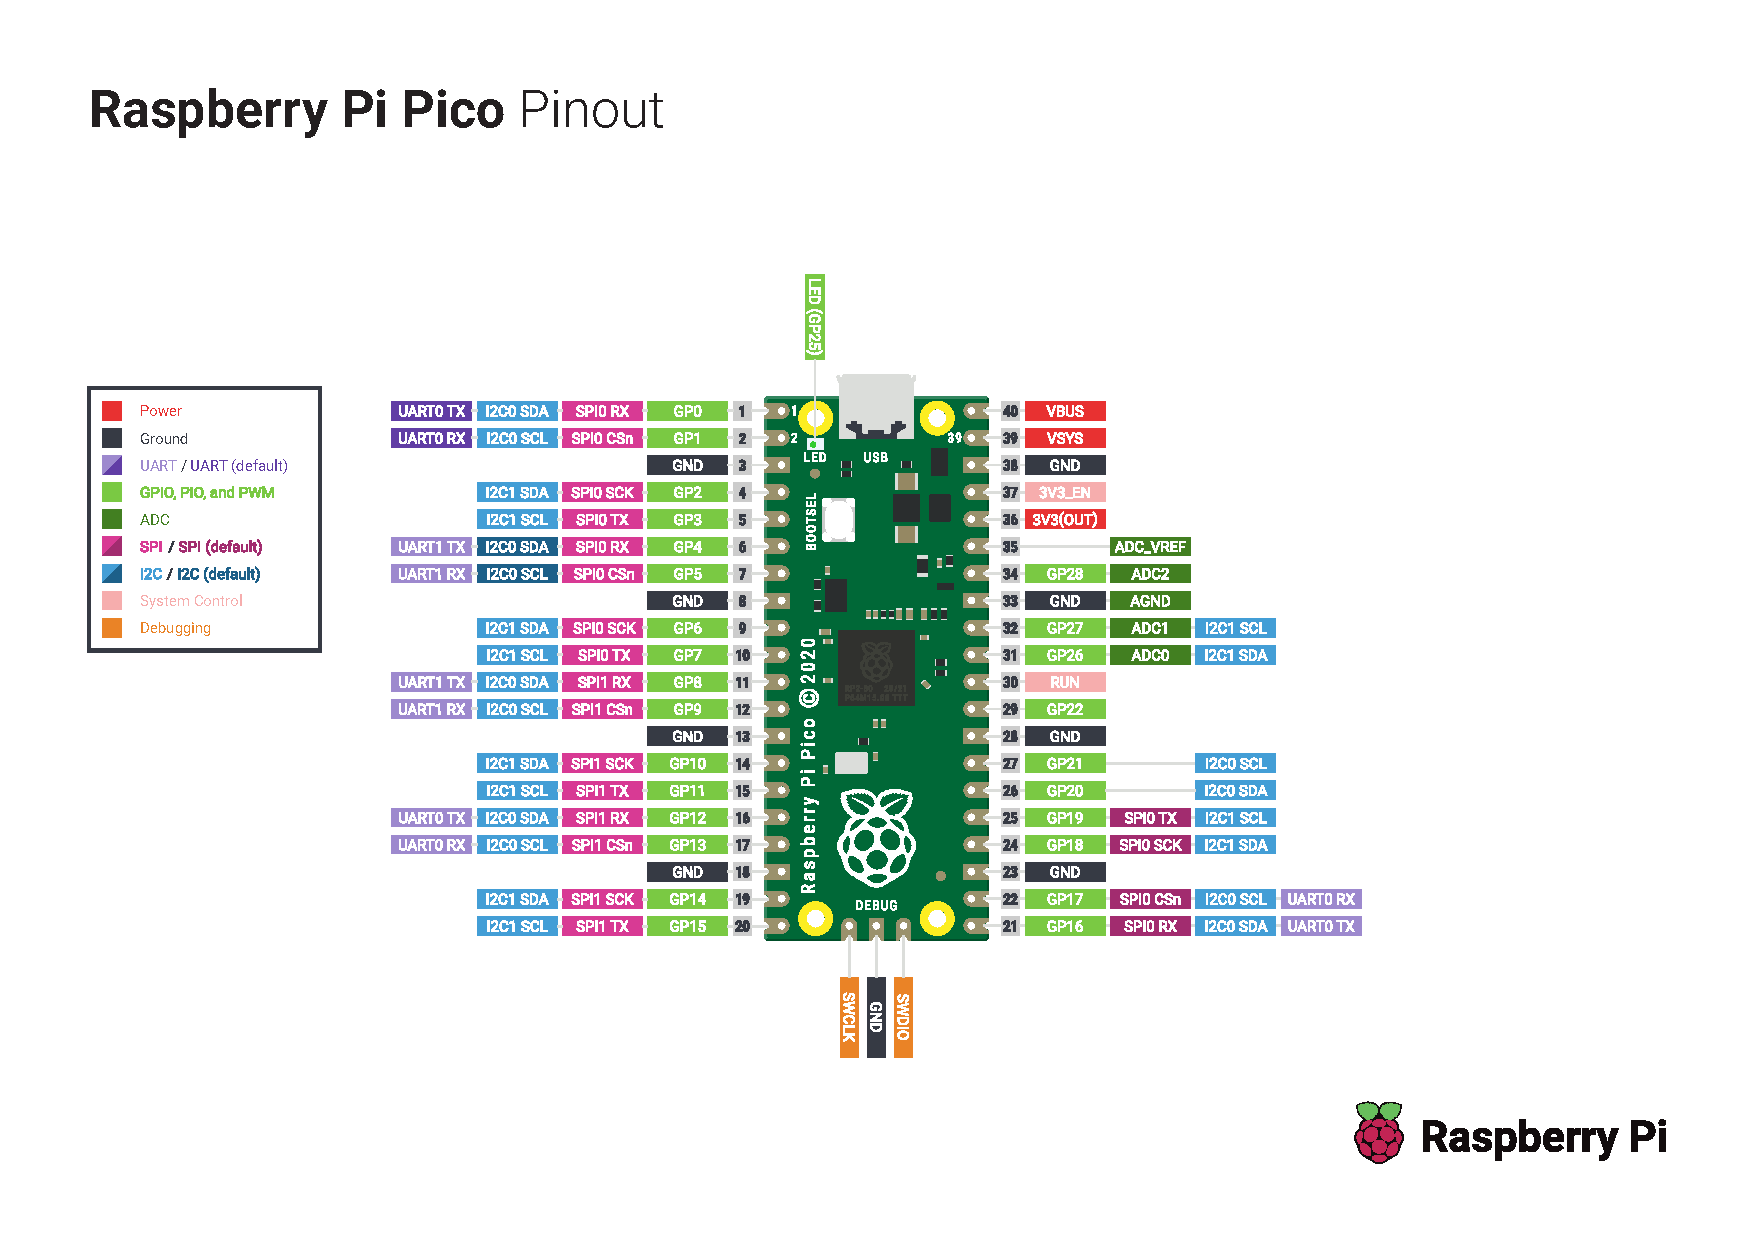
\includegraphics[width=\columnwidth]{Images/Pico-R3-A4-Pinout.pdf}
    \end{figure}

\section{Linear / Log Brightness Script}
    \begin{figure}[h]
        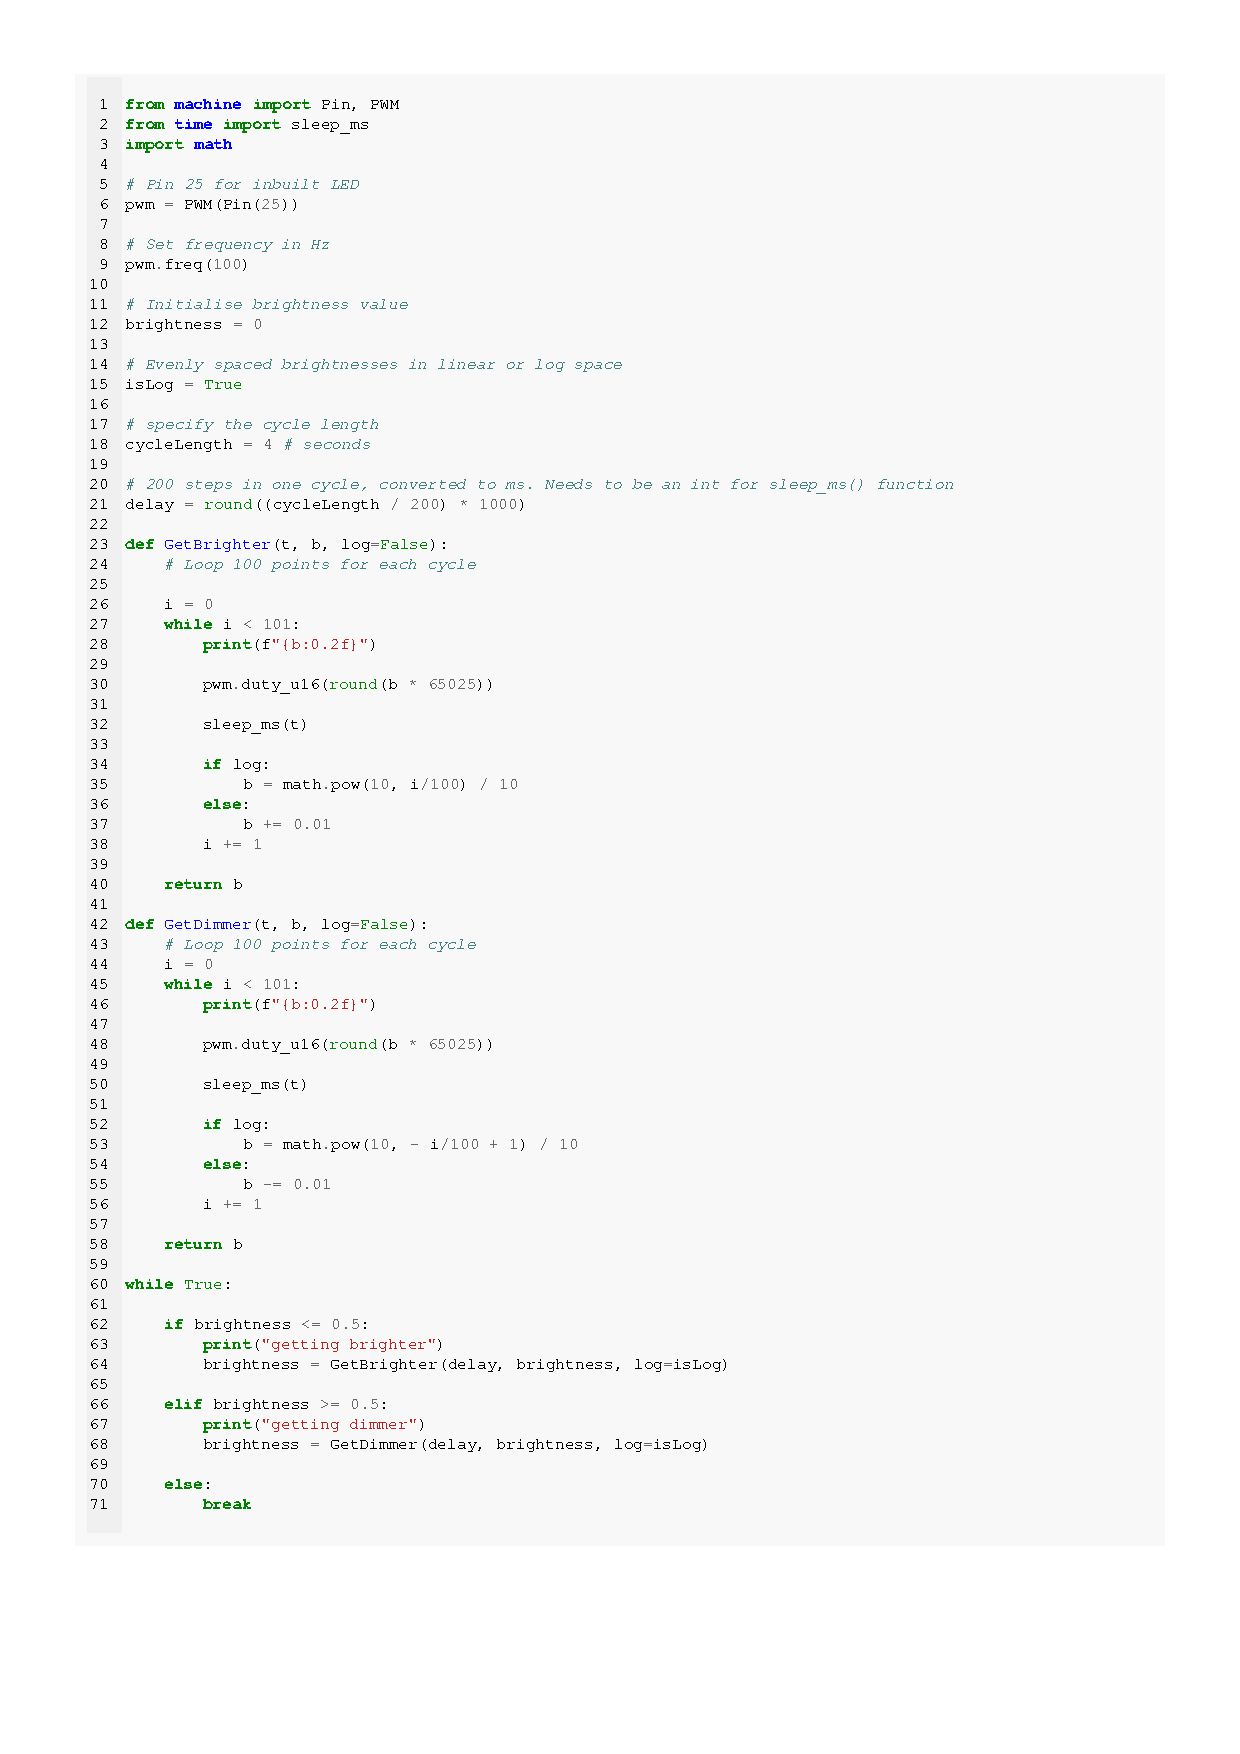
\includegraphics[width=\columnwidth]{Images/linearLogBrightness.pdf}
    \end{figure}


\clearpage
\section{Python Notebook}

\end{document}
%
% ****** End of file apssamp.tex ******
